% !TeX program = xelatex
% !TeX encoding = UTF-8
% !TeX root    = document_template.tex
\documentclass{../SIBGU-state}

\usepackage{multirow}
\usepackage{hyperref}
\hypersetup{pdftitle={Шаблон для курсовой}, pdfauthor={И. С. Скрябин}}

\usepackage{graphicx}

\begin{document}
	
\begin{titlepage}
	\pagestyle{empty}
	\setlength\parindent{0pt}
	\newcommand{\blankDate}[2]{\mbox{\uline{<<\makebox[.7cm]{#1}>>~\makebox[2cm]{#2}~\the\year{}~г.}}} % {день}{месяц}
	\newcommand\blankLine[2]{$\underset{\text{#1}}{\text{\uline{#2}}}$}
	\begin{center}
        \begin{footnotesize}
    		\textbf{МИНИСТЕРСТВО НАУКИ И ВЫСШЕГО ОБРАЗОВАНИЯ РОССИЙСКОЙ ФЕДЕРАЦИИ} \par 
    		Федеральное государственное бюджетное образовательное учреждение высшего образования \par\bigskip
        \end{footnotesize}
		\small\textbf{<<Сибирский государственный университет науки и технологий имени академика М.Ф. Решетнева>>} \par
        \bigskip
		\blankLine{институт}{Институт информатики и телекоммуникаций} \par
		\blankLine{кафедра}{Кафедра информатики и вычислительной техники} \par
		\bigskip\bigskip\bigskip\bigskip\bigskip\bigskip\bigskip
		{\fontsize{16pt}{16pt}\selectfont
			\textbf{КУРСОВАЯ РАБОТА}} \par
		по дисциплине \blankLine{дисциплина}{Базы данных}
	\end{center}
    \bigskip
    \begin{center}
        \blankLine{тема}{Разработка базы данных строительной организации} \bigskip\par
    \end{center}
    \bigskip\bigskip\bigskip\bigskip\bigskip\bigskip\bigskip\bigskip\bigskip\bigskip\bigskip\bigskip\bigskip\bigskip\bigskip
	Преподаватель {\hspace{5.4cm}} \hfill\blankLine{подпись, дата}{\hspace{3cm}} \hfill\blankLine{инициалы, фамилия}{О. Н. Лопатеева} \bigskip\bigskip\par
	Обучающийся \hfill\blankLine{номер группы, зачетной книжки}{БИМ21-01, 211213013}\hfill\blankLine{подпись, дата}{\hspace{3cm}} \hfill\blankLine{инициалы, фамилия}{И. С. Скрябин} \bigskip\par
	\begin{center}
		\vfill Красноярск~--- \the\year{}~г.
	\end{center}
	\newpage
    \begin{center}
        Институт информатики и телекоммуникаций \par
        Кафедра информатики и вычислительной техники \par
        \bigskip\bigskip\bigskip
        \fontsize{16pt}{16pt}\selectfont
		\textbf{ЗАДАНИЕ} \par
    \end{center}
	На курсовую работу по дисциплине \uline{\textit{Базы данных}} \smallskip\par
    Обучающемуся \uline{\textit{Скрябину Илье Сергеевичу}} \smallskip\par
    Группа \uline{\textit{БИМ21-01}}{\hspace{3cm}} Форма обучения \uline{\textit{Очная}} \smallskip\par
    Тема работы: \uline{\textit{Проектирование базы данных строительной организации,}}\par
    \uline{\textit{средствами СУБД MS SQL Server 2019}} \smallskip\par
    Срок сдачи курсовой работы \hfill\textit{\blankDate{30}{декабря}} \bigskip\par
    Перечень вопросов, подлежащих разработке при написании теоретической части: \par
    \uline{\textit{Анализ существующего программного обеспечения;}} \par
    \uline{\textit{Концептуальное проектирование базы данных;}} \par
    \uline{\textit{Логическое проектирование базы данных;}} \par
    \uline{\textit{Выбор целевой СУБД.}} \bigskip\par
    Перечень вопросов, подлежащих разработке при написании практической части: \par
    \uline{\textit{Физическое проектирование базы данных;}} \par
    \uline{\textit{Структура программного продукта;}} \par
    \uline{\textit{Руководство программиста;}} \par
    \uline{\textit{Краткое руководство пользователя.}} \bigskip\par
    \bigskip\bigskip\bigskip
    Дата выдачи задания \hfill\textit{\blankDate{1}{октября}} \bigskip\par
	Задание на курсовую работу выдал \blankLine{инициалы, фамилия}{\textit{О. Н. Лопатеева}} \hfill\blankLine{(подпись руководителя)}{\hspace{3cm}} \par
	Задание на курсовую работу получил \blankLine{инициалы, фамилия}{\textit{И. С. Скрябин}} \hfill\blankLine{(подпись обучающегося)}{\hspace{3cm}} \par\bigskip
	\begin{center}
		Красноярск~--- \the\year{}~г.
	\end{center}
\end{titlepage}
\addtocounter{page}{2}


\tableofcontents



\section*{Введение}
\phantomsection
\addcontentsline{toc}{section}{Введение}

\textit{Актуальность:}\par
В наше время огромное количество фирм используют персональные компьютеры для сохранения и обработки любого вида информации. Эта информация содержится в базах данных. Базы данных играют важную роль в развивающемся мире технологий. Всё, с чем мы каждый день взаимодействуем в жизни, по всей видимости, зафиксировано в какой-нибудь базе. Работа с базами данных является важнейшим навыком в работе с компьютером, а специалисты данной области становятся всё более востребованными. Главные идеи нынешней информационной методики базируются на представлении, в соответствии чему информация должна быть образована в базы данных с задачей отображения динамически изменяющегося мира и удовлетворения всех потребностей в информации у пользователей. Базы данных формируются и работают под управлением специальных программных средств, называемых системами управления базами данных.\par\bigskip
\textit{Цель и задачи:}\par
 Главная цель данной курсовой работы заключается в осуществлении концептуального, логического и физического проектирования базы данных для конкретной организации, а также разработке приложения с интуитивным интерфейсом и расширенными функциями для взаимодействия с данной базой данных. В процессе выполнения курсовой работы будут решаться следующие задачи:
\begin{itemize}
	\item провести анализ ПО в области строительства;
	\item провести концептуальное проектирование базы данных;
    \item спроектировать логическую модель базы данных;
	\item осуществить выбор СУБД и выполнить физическое проектирование базы данных;
    \item разработать приложение для работы с базой данных, составить руководство пользователя по работе с приложением;
	\item протестировать разработанное приложение для взаимодействия с базой данных.
\end{itemize}\par\bigskip\bigskip
\textit{Структура работы:}\par
В главе 1 курсовой работы представлен обзор ПО для автоматизации строительных организаций, концептуальное и логическое проектирование базы данных, выбор целевой СУБД для создания базы данных и физическое проектирование базы данных в выбранной СУБД.\par
Глава 2 курсовой работы состоит из пунктов с описанием структуры ПО, функциях работы ПО и краткого руководства пользователя.\par\bigskip


\section{Теоретическая часть}

\subsection{Анализ существующего программного обеспечения}

На сегодняшний день на рынке ПО в сфере строительства существует множество различных продуктов для учета данных о заказчиках, материалах, строительстве и т.д. Множество из них похожи между собой функционалом, но можно выделить 4 самых крупных и известных программных продукта:
«Gectaro», «Smetter», «Аспро.Cloud» и «АЛТИУС». В таблице 1 приведены характеристики ПО от каждой компании:
\begin{table}[htb]
	\caption{Таблица в~приложении}
	\centering
	\small\begin{tabular}{ |p{4.7cm}|c|c|c|c| }
        \hline
		Критерий &«Gectaro» & «Smetter» & «Аспро.Cloud» & «АЛТИУС» \\ \hline
        Русский язык & + & + & + & + \\ \hline
        Простой интерфейс & + & + & + & + \\ \hline
        Быстрый доступ к требуемой информации & + & + & + & - \\ \hline
        Расчет параметра в процессе заполнения & + & - & + & - \\ \hline
        Фильтрация данных по критериям & + & + & + & + \\ \hline
        Дата выхода последней версии & 2023г & 2022г & 2022г & 2021г \\ \hline
        Стоимость & 35000руб/мес & Неизвестна & Неизвестна & Неизвестна \\ \hline
	\end{tabular}
	\label{tab:in_appendix}
\end{table}\par
В ходе проведения анализа ПО каждой компании были выявлены преимущества и недостатки каждого отдельного продукта. Однако следует заметить, что не во всех продуктах присутствует «расчет параметра в процессе заполнения», поскольку в сфере строительства скорее важен учет материалов и процессы выполнения работы по постройкам. \par
Поскольку все единые цифровые платформы (ЕЦП) разработаны в РФ и, соответственно, имеют русскую локализацию, их создатели стараются создавать простой интерфейс, удобный для сотрудников строительных организаций, а также регулярно обновлять свои продукты. Логично следует, что большинство программных продуктов схожи по функционалу и выбор в использовании конкретной программы остается за самой организацией. \par

\subsection{Концептуальное проектирование базы данных}
Чтобы создать базу данных, нужно сначала концептуально спроектировать ее. Для этого выделим все необходимые сущности, связи в таблице 2, и представим их диаграммы в таблице 3. \par
\begin{table}[htb]
	\caption{Сведения о типах сущностей}
	\centering
	\small\begin{tabular}{ |p{2cm}|p{3.5cm}|p{5.4cm}|p{4cm}| }
        \hline
		№ & Имя сущности & Описание & Тип \\ \hline
        1 & Строители & Содержит информацию о строителях. Ключ – порядковый номер строителя. & Сильная \\ \hline
        2 & Виды строительства & Содержит информацию о видах строительства. Ключ – порядковый номер вида строительства. & Сильная \\ \hline
        3 & Заказчики & Содержит информацию о заказчиках. Ключ – порядковый номер заказчика. & Сильная \\ \hline
        ... & ... & ... & ... \\ \hline
	\end{tabular}
	\label{tab:in_appendix}
\end{table}\par

\begin{table}[htb]
	\caption{Сведения о связях}
	\centering
	\small\begin{tabular}{ |p{1.6cm}|p{3.5cm}|p{3.4cm}|p{3cm}|p{3cm}| }
        \hline
		№ & Первая сущность & Связь & Вторая сущность & Кардинальность \\ \hline
        1 & Строители & Участвуют в & Консультациях & 1:M \\ \hline
        2 & Строители & Работают по & Времени работы & M:1 \\ \hline
        3 & Строители & Привязаны к & Офису & M:1 \\ \hline
        ... & ... & ... & ... & ...\\ \hline
	\end{tabular}
	\label{tab:in_appendix}
\end{table}\par

Изобразим ER-диаграммы для каждой сущности и их связи, которые показаны на рисунках 1-16: \par
\begin{figure}[htb]
	\centering
	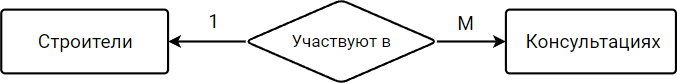
\includegraphics[width=1\textwidth]{ris/ris1.png}
	\parskip=1pt
	\caption{ER-диаграмма связи 1}
	\label{fig:in_appendix}
\end{figure}\par
И так далее...\par\bigskip
Соединив все построенные ER-диаграммы связей, получаем общую ER диаграмму связей для всех сущностей базы данных, показанной на рисунке 17 (в шаблоне это рисунок 2): \par
\begin{figure}[htb]
	\centering
	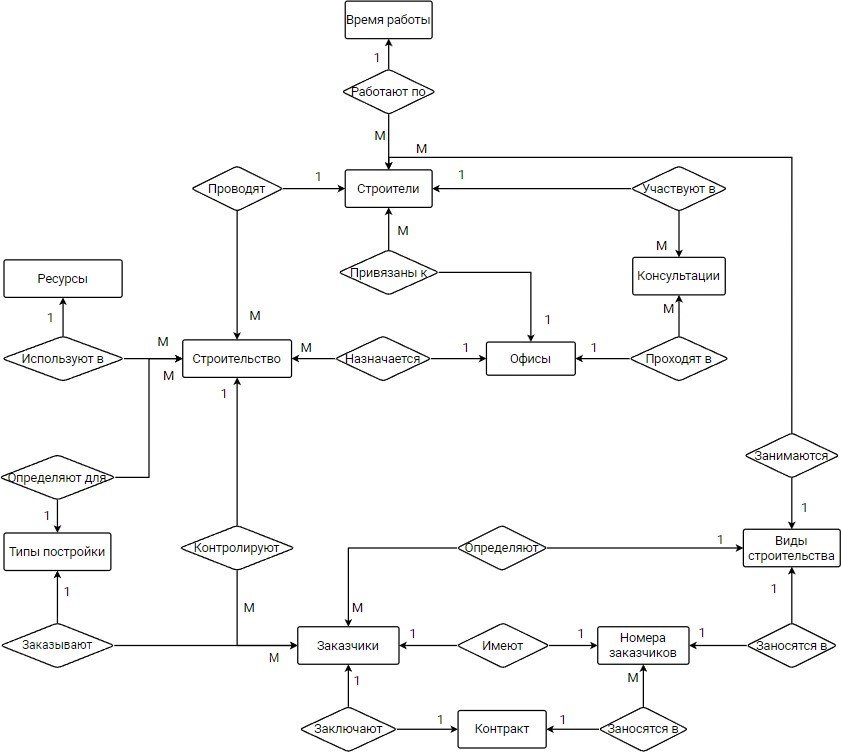
\includegraphics[width=1\textwidth]{ris/ris2.jpg}
	\parskip=1pt
	\caption{Общая ER-диаграмма связей}
	\label{fig:in_appendix}
\end{figure}\par

Сформируем для каждой связи предварительные отношения с указанием первичного ключа: \par
\begin{enumerate}[label=\asbuk*), ref=\asbuk*]
    \item[] Связь 1 (Строители-Консультации):
	\item Строители (Номер строителя).
	\item Консультации (Номер консультации, номер строителя) – добавляется ключевой атрибут «номер строителя».
\end{enumerate}\par\bigskip
\begin{enumerate}[label=\asbuk*), ref=\asbuk*]
    \item[] Связь 2 (Строители-Время работы):
	\item Строители (Номер строителя, номер консультации).
	\item Время работы (Номер времени работы, номер строителя) – добавляется ключевой атрибут «номер строителя».
\end{enumerate}\par\bigskip
И так далее...\par\bigskip
Также добавляем в отношения не ключевые атрибуты:\par
\begin{itemize}
	\item Строители (Номер строителя, Имя, Фамилия, Отчество, Дата рождения, Номер офиса, Специализация);
	\item Консультации (Номер консультации, Номер офиса, Номер строителя, Номер заказчика, Дата консультации);
    \item Виды строительства (Номер вида строительства, Наименование вида строительства, Номер строителя, Номер заказчика, Номер мобильного телефона).
\end{itemize}\par\bigskip
И так далее...\par\bigskip

Учитывая	выявленные	атрибуты,	составляем	ER-диаграмму экземпляров, которая продемонстрирована на рисунке 18 (в шаблоне это рисунок 3): \par
\begin{figure}[htb]
	\centering
	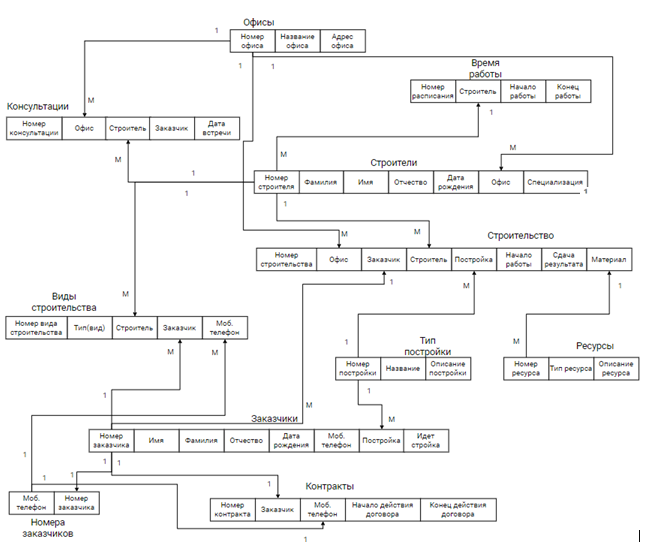
\includegraphics[width=1\textwidth]{ris/ris3.png}
	\parskip=1pt
	\caption{Общая ER-диаграмма экземпляров}
	\label{fig:in_appendix}
\end{figure}\par

\subsection{Логическое проектирование базы данных}

При логическом проектировании базы данных была выполнена нормализация до 3 уровня НФ (нормальной формы). Были сформированы справочные таблицы и составлена диаграмма логической модели базы данных на рисунке 19 (в шаблоне это рисунок 4), а сведения об атрибутах сущностей представлены на таблице 4: \par
\begin{figure}[htb]
	\centering
	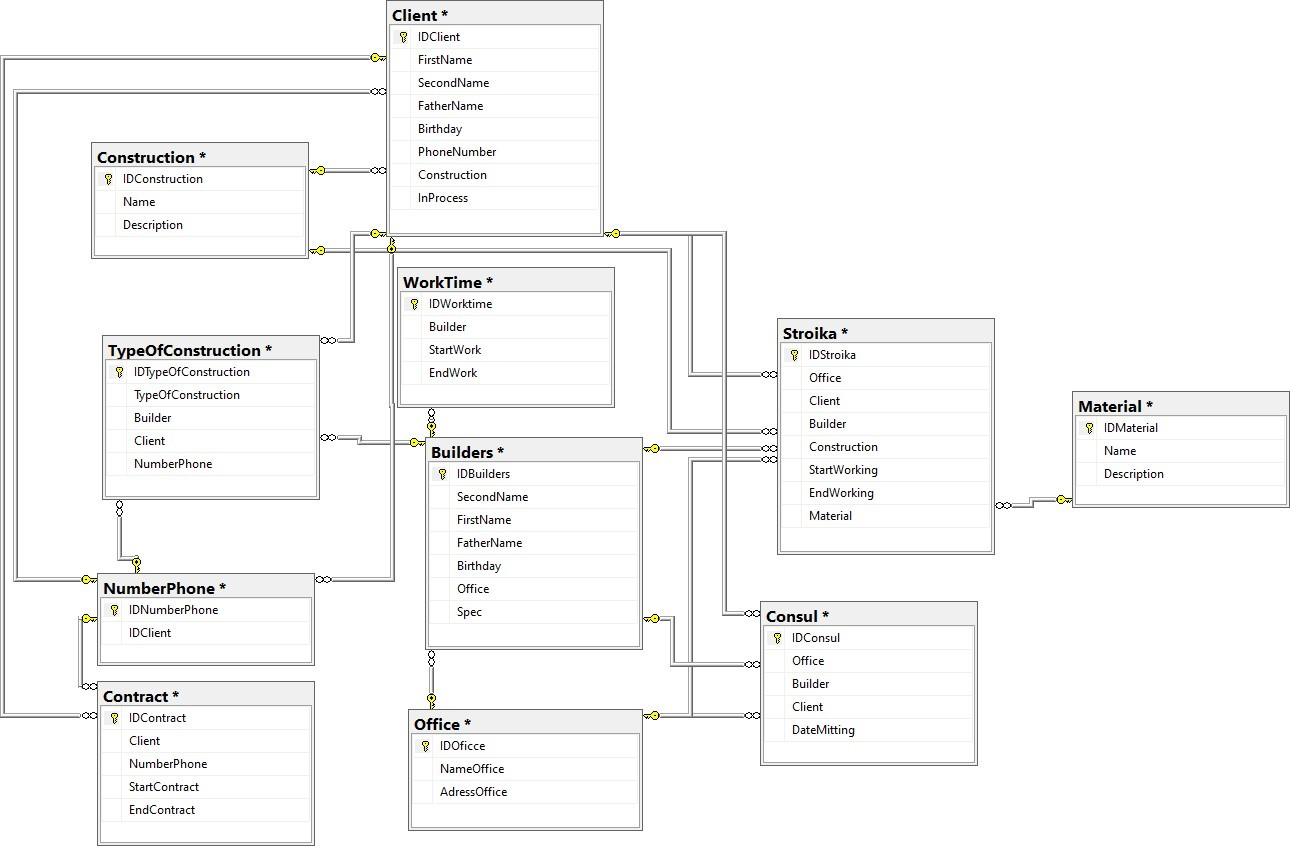
\includegraphics[width=1\textwidth]{ris/ris4.jpg}
	\parskip=1pt
	\caption{Диаграмма логической модели базы данных}
	\label{fig:in_appendix}
\end{figure}\par
\begin{table}[htb]
	\caption{Сведения об атрибутах сущностей}
	\centering
	\small\begin{tabular}{ |p{3.6cm}|p{4.1cm}|p{3.8cm}|p{3cm}| }
        \hline
		Сущность & Наименование атрибута & Атрибут сущности & Домен атрибута \\ \hline
        \multirow{1}{*}{\parbox[t]{5cm}{Строители \\ (Builders)}} & IDBuilders & Идентификатор строителя & Числовой\\
        \cline{2-4}
        & FirstName & Имя & Текстовый\\
        \cline{2-4}
        & SecondName & Фамилия & Текстовый\\
        \cline{2-4}
        & FatherName & Отчество & Текстовый\\
        \cline{2-4}
        & Birthday & Дата рождения & Дата\\
        \cline{2-4}
        & Office & Номер офиса & Числовой\\
        \cline{2-4}
        & Spec & Специализация & Текстовый\\
        \hline
        \multirow{2}{*}{\parbox[t]{5cm}{Виды строительства \\ (TypeOfConstruction)}} & IDTypeOfConstruction & Идентификатор Вида стройки & Числовой\\
        \cline{2-4}
        & TypeOfConstruction & Наименование Вида стройки & Текстовый\\
        \cline{2-4}
        & Builder & Номер строителя & Числовой\\
        \cline{2-4}
        & Client & Номер заказчика & Числовой\\
        \cline{2-4}
        & NumberPhone & Номер мобильного & Числовой\\
        \hline
        ... & ... & ... & ... \\
        \hline
	\end{tabular}
	\label{tab:in_appendix}
\end{table}\par

\subsection{Выбор целевой СУБД}
Перед тем, как приступить к физическому проектированию, нужно выбрать СУБД. Для подробного анализа рассмотрим следующие СУБД: \par
\begin{enumerate}
	\item \textit{Microsoft SQL Server} — система управления реляционными базами данных, разработанная корпорацией \textit{Microsoft};
	\item \textit{MySQL} — свободная реляционная система управления базами данных;
    \item \textit{MongoDB}— не реляционная система управления базами данных (\textit{NoSQL}), в которой для хранения данных используются документы.
\end{enumerate}
Сравнение выбранных СУБД представлено в таблице 5: \par
\begin{table}[htb]
	\caption{Сведения о типах сущностей}
	\centering
	\small\begin{tabular}{ |p{2cm}|p{3.5cm}|p{5.4cm}|p{4cm}| }
        \hline
		Критерий сравнения & \textit{Microsoft SQL Server} & \textit{MySQL} & \textit{MongoDB} \\ \hline
        Логическая модель данных & Реляционная & Реляционная & Не реляционная \\ \hline
        Физическая модель данных & Страничная & Страничная & Страничная \\ \hline
        Тип данных & Все основные & Все основные & Все основные \\ \hline
        ... & ... & ... & ... \\ \hline
	\end{tabular}
	\label{tab:in_appendix}
\end{table}\par
В процессе анализа СУБД были обнаружены плюсы и минусы каждой рассмотренной базы данных. Исходя из информации в таблице 5, можно сделать вывод о том, что \textit{Microsoft SQL Server} является более универсальной и подходящей для проектирования в рамках учебных проектов.

\subsection{Физическое проектирование базы данных}
При физическом проектировании базы в СУБД \textit{«Microsoft SQL Server 2019»} были реализованы таблицы базы данных. \par
\textit{Таблицы в БД} - это объекты базы данных, предназначенные для хранения пользовательских данных. \par
Описание таблиц БД «BuildBD» представлено в таблицах 6-16: \par\bigskip
Также составляем таблицы, по типу тех, которые были реализованы ранее. Полный документ в том числе и содержание таблиц 6-16, вы можете увидеть в документе \textit{«Курсовая Скрябин.docx»}. \par

\section{Практическая часть}

\subsection{Структура программного продукта}
В программном продукте имеется 11 вкладок, среди которых одна является главной, а остальные можно выбирать через соответствующее меню. Каждая вкладка содержит таблицу, которая основана на спроектированной базе данных: \par
\begin{itemize}
	\item Строители (\textit{главная вкладка});
	\item Время работы;
    \item Офисы;
    \item Консультации;
    \item Заказчики;
    \item Номера телефонов;
    \item Контракты;
    \item Тип постройки;
    \item Материалы/ресурсы;
    \item Виды строительства;
    \item Строительство.
\end{itemize}\par\bigskip

\subsection{Функции программного продукта}
Программа была создана с использованием языка программирования C\# в среде разработки Visual Studio 2022. Хранение данных осуществляется в базе данных, которая работает на СУБД «Microsoft SQL Server Management Studio 2019». В приложении доступны следующие возможности: \par
\begin{itemize}
	\item Вывод таблиц из базы данных на каждую соответствующую таблицу DataGridView во вкладке;
	\item Добавление, редактирование и удаление кортежей таблицы;
    \item Перемещение по кортежам таблицы в специальной панели инструментов;
    \item Сортировка таблицы по любому столбцу;
    \item Строка поиска для фильтрации кортежей по введенному запросу для любого столбца;
    \item Обновление данных всех вкладок с соответствующими таблицами;
    \item Сохранение введенных изменений в файл БД.
\end{itemize}\par\bigskip

\subsection{Краткое руководство пользователя}
В верхней части окна приложения расположена панель управления, на которой находятся кнопки для переключения между кортежами таблицы, добавления и удаления кортежей, сохранения таблицы в текущей открытой вкладке и обновления всех таблиц базы данных.\par 
Окно приложения и панель управления представлены на рисунках 20 и 21 (в данном случае 5 и 6): \par
\begin{figure}[htb]
	\centering
	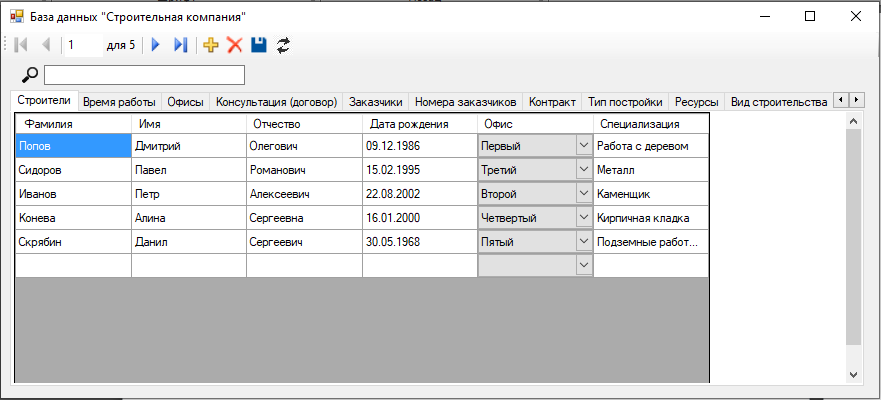
\includegraphics[width=.9\textwidth]{ris/ris5.png}
	\parskip=1pt
	\caption{Окно приложения базы данных «Строительная компания»}
	\label{fig:in_appendix}
\end{figure}\par
\begin{figure}[htb]
	\centering
	
\includegraphics[width=.5\textwidth]{ris/ris6.jpg}
	\parskip=1pt
	\caption{Панель управления приложения}
	\label{fig:in_appendix}
\end{figure}\par
Пример перемещения между строками таблицы: \par
При смене вкладок курсор всегда будет находиться на первой строке открытой таблицы. Чтобы переместить курсор на следующую или предыдущую вкладку, нажмите соответствующие кнопки. Для перемещения на первую или последнюю строку таблицы используйте кнопки на панели управления.\par\bigskip
Пример переключения между строками показан на рисунке 22:\par
Далее расписываем функционал программы, используя скриншоты самой программы, с полным описанием функционала можете ознакомиться в документе «Курсовая Скрябин.docx». \par


\section*{Заключение}
\phantomsection
\addcontentsline{toc}{section}{Заключение}

В процессе выполнения курсовой работы были выполнены следующие типы задач: \par
\begin{itemize}
	\item проведен анализ программного обеспечения в сфере строительства;
	\item произведено концептуальное проектирование базы данных, где будут храниться данные;
    \item осуществлено логическое проектирование базы данных;
    \item произведен выбор СУБД и осуществлено физическое проектирование базы данных;
    \item разработана архитектура приложения, обеспечивающего ведение учета в строительной организации;
    \item создано руководство программиста и руководство для пользователя;
    \item проведено тестирование разработанного приложения.
\end{itemize}\par\bigskip
Во время создания курсовой работы по теме «Создание базы данных строительной организации» было проведено глубокое изучение материалов (литература, видеоролики), где объясняются и раскрываются теоретические вопросы и ключевые понятия данного исследования, а также сделан анализ практического применения баз данных. \par
Автоматизация сбора и хранения информации о проектах в организации существенно улучшает эффективность рабочего процесса, сокращая количество данных (которые не были обработаны вовремя), а также снижая затраты времени. \par
Реализованная программа содержит в себе все нужные функции. \par


\begin{thebibliography}{99\kern\bibindent}
	\bibitem{bib:mybook} Windows Forms. Программирование на C\# [Электронный ресурс]. ~--- Режим доступа: \url{http://csharpcoding.org/category/windows-forms/} (дата обращения: 01.11.2023). ~--- Текст: электронный.
	\bibitem{bib:mybook2} Основы использования и проектирования баз данных. / Илюшечкин В.М. ~--- 2020г. 214 с. ~--- Текст : непосредственный. 
    \bibitem{bib:mybook3} «Руководство по ADO.NET и работе с базами данных, Глава 2. C\# и «MS SQL Server» ~--- Metanit [сайт]. ~--- URL: \url{ https://metanit.com/sharp/adonet/2.1.php} (дата обращения 21.10.2023). ~--- Текст: электронный. 
    \bibitem{bib:mybook4} Малыхина, М.П. Базы данных: основы, проектирование, использование / М.П. Малыхина. ~--- СПб.: BHV, 2007. ~--- 528 c. ~--- Текст: непосредственный. 
\end{thebibliography}



\appendix

\section{Техническое задание на разработку}

Введение: \par
В настоящее время многие компании стремятся заменить традиционную бумажную отчетность на электронную форму, и строительные организации не являются исключением. В связи с этим разработка базы данных для строительных организаций и создание соответствующего программного обеспечения были выбраны в качестве задачи для разработки. \par\bigskip

Общие положения: \par
\textit{Полное наименование:} Проектирование базы данных строительной организации.\par
\textit{Краткое наименование:} «BuildDB».\par
\textit{Разработчик:} Скрябин Илья Сергеевич, группа БИМ21-01\par
\textit{Вид разработки:} Проектирование базы данных и разработка программы.\par
\textit{Основание для разработки:} Разработка программного продукта ведется на основании учебного плана СибГУ им. М.Ф. Решетнева по направлению подготовки 09.03.01 «Программное обеспечение мобильных систем и приложений».\par
\textit{Плановые сроки начала и окончания выполнения работы:} \par
Плановый срок начала работ по «BuildDB» – 01.10.2023 \par
Плановый срок окончания работ по «BuildDB» – 21.12.2023\par
\textit{Назначение	разработки:}	Разрабатываемый	программный	продукт предназначен для учета объектов строительной организации.\par\bigskip

Требования к программе:\par
\textit{Требования к функциональным характеристикам:}\par
В программе должно быть предусмотрено представление:\par
\begin{itemize}
	\item Информации по всем строителям;
	\item Информации по всем временам работы;
    \item Информации по всем офисам;
    \item Информация по всем консультациям;
    \item Информации по всем заказчикам;
    \item Информации по всем номерам заказчиков;
    \item Информации по всем контрактам;
    \item Информации по всем типам построек;
    \item Информации по всем материалам/ресурсам;
    \item Информации по всем видам строительства.
\end{itemize}\par
\textit{Программа должна:}\par
\begin{itemize}
	\item обеспечить пользователю возможность получить требуемую информацию на экран в простой форме и легком доступе;
	\item позволять просматривать, редактировать и удалять информацию.
\end{itemize}\par
Необходимо обеспечить возможность ввода данных в программе с помощью заполнения таблиц или специальных форм. Информация должна выводиться на экран в виде текстовых таблиц или текста на форме.\par
\textit{Требования к надежности:}\par
Необходимо реализовать механизм контроля за добавлением, удалением и изменением данных в программе. Важно, чтобы любые внутренние ошибки не приводили к потере данных. Программа должна информировать о возникших ошибках и предупреждать о действиях, которые могут привести к потере данных.\par
\textit{Условия эксплуатации:}\par
Приложение рассчитано на эксплуатацию пользователями строительных организаций.\par
\textit{Требования к составу и параметрам технических средств:}\par
\begin{itemize}
	\item система должна работать под управлением семейства операционных систем Win64 (Windows 7/8/10/Server 2012 и выше);
	\item наличие на ПК установленной SQL Server 2019 и выше;
    \item минимум 100 Мб свободного места на диске.
\end{itemize}\par
\textit{Требования к информационной и программной совместимости:}\par
\begin{itemize}
	\item операционная система Windows 7/8/10;
	\item среда разработки Visual Studio 2022;
    \item СУБД «Microsoft SQL Server 2019»;
    \item Microsoft Office.
\end{itemize}\par\bigskip\bigskip\bigskip

Состав и содержание работ по выполнению курсовой работы:\par
\begin{table}[htb]
	\caption{Календарный план-график выполнения стадий и этапов разработки}
	\centering
	\small\begin{tabular}{ |p{10cm}|p{4.9cm}| }
        \hline
		\textbf{\textit{Наименование работ}} & \textbf{\textit{Сроки выполнения}} \\ \hline
        Анализ предметной области & 03.10.2023 \\ \hline
        Обзор аналогичного программного обеспечения & 10.10.2023\\ \hline
        Концептуальное проектирование базы данных & 11.10.2023\\ \hline
        Логическое проектирование базы данных & 18.10.2023\\ \hline
        Выбор целевой СУБД & 29.10.2023\\ \hline
        Физическое проектирование базы данных & 09.11.2023\\ \hline
        Разработка структуры & 16.11.2023\\ \hline
        Разработка пользовательского интерфейса & 28.11.2023\\ \hline
        Программная реализация & 07.12.2023\\ \hline
        Тестирование и отладка & 17.12.2023\\ \hline
        Оформление пояснительной записки & 21.12.2023\\ \hline
        Предоставление преподавателю результатов работы & 30.12.2023\\ \hline
	\end{tabular}
	\label{tab:in_appendix}
\end{table}\par


\section{Общая информация о шаблоне}

Полное содержание работы, на которой было основано проектироание данного шаблона, вы можете увидеть в файле «Курсовая Скрябин.docx». \par
Здесь же я продемонстрировал основные функции работы с XeLaTeX, используя которые, вы можете написать своб собственную курсовую работу. \par
Также более подробные теоритические указания по работе с командами LaTeX есть в файле «documentation.tex» и «listings.tex». \par
Стили меняются в файле «SIBGU-state.cls». \par


	
\end{document}